\documentclass[12pt,a4paper,twocolumn]{article}
\usepackage[latin1]{inputenc}
\usepackage{amsmath}
\usepackage{amsfonts}
\usepackage{amssymb}
\usepackage{textcomp}
\usepackage{graphicx} 
\author{Alexandros-Panagiotis Oikonomou}
\title{Image Contour Extraction}
\begin{document}
\maketitle
\newpage
\thispagestyle{empty}
\mbox{}
\newpage
\thispagestyle{empty}
\mbox{}
\newpage
\thispagestyle{empty}
\mbox{}
\section{Introduction}
For the assignement of the Intelligent Algorithms course I was asked to implement an Image Contour Extractor algorithm. With the use of MATLAB the principle of Dynamic Programming was adopted for the implementation. Throughout this report the design of the algorithm is documented along with findings made by testing the algorithm. 
\section{Program Design}
This section will describe the design used in order to implement the algorithm.
\subsection{Search Space}
The design to extract the search space has been kept into a fairly simple level. There exists a function search\_space which takes as arguments the image matrix returned by the imread command and the contour initialisations. It returns a 3D Matrix of type (rows(image),M,3) called points, where M is the number of rows the user wishes to have inside the search space. In the first index (i,j,1) the x value of the image is kept, in the second index (i,j,2) the y value of the image is stored and in the third index (i,j,3) the intensity of the of (x,y) point is stored. That way each (i,j) point in the points matrix correspons to an (x,y) value of the image. Before the matrix is returned the values of the intensities are negated.
\subsection{Dynamic Programming}
In order to apply the algorithm supplied in the assignement there exists a function get\_energies which takes as arguments the image matrix, the two initialisation contours and the lambda that the user wishes to choose. The first command is to call the search space function mentioned above. As output parameters it returns a energy matrix, a position matrix and matrix returned by the search space called intensity. The intensity matrix is returned in order to be used for backtracking. The energy matrix is a 3D matrix of the form (rows(intensity),columns(intensity),rows(intensity)). 

The first two terms are there to correspond to the same point as in the intensity matrix. For all the points in the previous column, depending on the point the algorithm is currenlty at, the minimum energy of all the points in the previous column is stored in the last term of the energy matrix. 
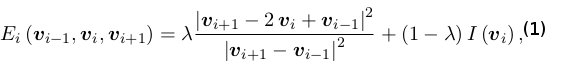
\includegraphics[width=250pt,height=50pt,scale=1]{energy_eq.jpg}
The reason it is a vector is that the above action is done for all the points of the next column of the point the algorithm is currently at. The energy is computed according to (1). 
The position matrix has the same first two terms, but the difference is in the third term, where the row of the minimum energy was found is stored, instead of the value itself. The result of computing energies of all these points is that a quadruple for-loop is used
\subsection{Backtracking}
The backtracking is completed in a function called get\_contour which returns the points of the contour\. The first calculations of this function locates the minimum energy along with its row and depth index in all the vectors of the next to last column. The reason this column is picked is that in the last column the computation is not completed in its entirety, due to the fact that there is no next column to do the computation correctly see (1). The algorithm now jumps to the node with the row index returned and the depth index in the position matrix and reads the value. Then the optimal path is chosen, by going to the next column by selecting the row, from the value returned before. The depth is found from the row index of that value.
\subsection{Negating Images}
It is also noteworthy to mention that the intensities of the points are negated before passed on to the produce\_energies function. The reason for that is that the algorithm searches and stores the minimum energy. That means that lower intensities are desired. The problem with the returned image, when applying the imread function, is that pixels which seem to be blacker have lower intensities and pixels which seem to be whiter seem to have higher intensities. By negating the intensities, this property is reversed and hence the algorithm searches for pixels wich seem whiter. Negating the image is done by the function negating\_intensities.
\section{Algorithm Testing}
This section will report the findings of applying the algorithm in different situations.
\subsection{Initial Results}
The initial test of the algorithm was to be done in a picture supplied by the assignement. The picture was of a X-ray of a tongue. The testing configuration asked was to be with $\lambda$=0.5. However M was bot specified so I chose M=100. The result contour displayed all but one points of the contour to lie perfectly on the outline of the tongue(5.1 Appendix).
\subsection{Scalability with changes in M}
\subsection{Robustness with changes in Lambda}
Changing $\lambda$ seemed to make the contour behave differently on certain occasions. 
It was observed that for 0.1 $<$ $\lambda$ $<$0.7 the contour did not seem to change significantly. It remained the same as it was for $\lambda$=0.5, with having most of the points lying in the tongue outline, but having one point in a completely different point. The picture resembled the one in 5.1(Appendix).
On the contrary for 0.8 $<$ $\lambda$ $<$0.9 it was observed that this point would now lie in the tongue, adjacent with the rest of the contour points. This made the contour more precise and accurate(5.2.1 Appendix).
Finally, a $\lambda$'=0.00001 was tested in order to identify any irregularities that may be caused for small values of $\lambda$'s. Again most of the points lied on the tongue, but this time in addition to the one irregular point that existed in previous $\lambda$'s there were some additional irregular points in the initial x's(5.2.2 Appendix). This can be attributed to the fact that with low $\lambda$'s emphasis is given in the intensity of the points and the intensity is found high at these points.
\subsection{Different contour initialisations}
To identify the strength of the algorithm, different initialisations of contours were tested.Initially, the first change was to move the top and bottom contours relative to the y-axis. Initial contour with higher top contour was tested(5.3.1 Appendix) and it was verified that the final contour would still be correctly drawn. The reason for that was that the intensities of the added search space were more or less the same as before, which resulted into having a precise contour. Next a lower bottom initial contour was chosen(Appendix 5.3.2). This time it is apparent that the contour breaks badly, even though some points still lie in the tongue outline. The reason for that is that points above the bottom contour have lower intensities than those that lie on the tongue. That makes the backtracking algorithm to choose them instead of the one on the tongue.
Finally
\subsection{Other tested images}
\section{Conclusion}
as
\newpage
\mbox{}

\newpage
\mbox{}
\section{Appendix}
\subsection{Initial result}
$\lambda=0.5$ and M=100
\newline
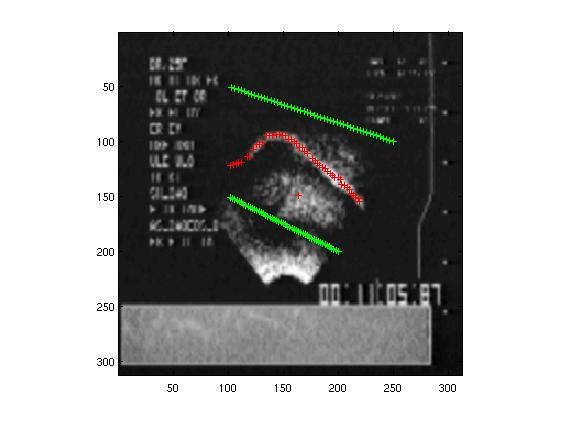
\includegraphics[width=500pt,height=400pt,scale=1]{points_1_to_7.jpg}
\newpage
\mbox{}
\newpage

\subsection{Tweaking $\lambda$'s}
\subsubsection{High $\lambda$'s}
0.8$<$ $\lambda$ $<$0.9 and M=100
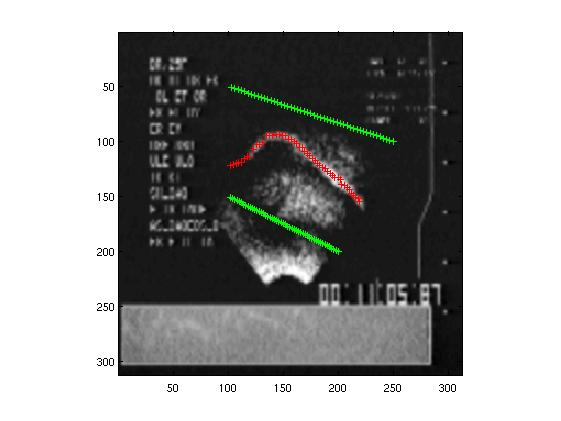
\includegraphics[width=500pt,height=400pt,scale=1]{89.jpg}
\newpage
\mbox{}
\newpage
\subsubsection{Low $\lambda$'s}
$\lambda$=0.00001 and M=100
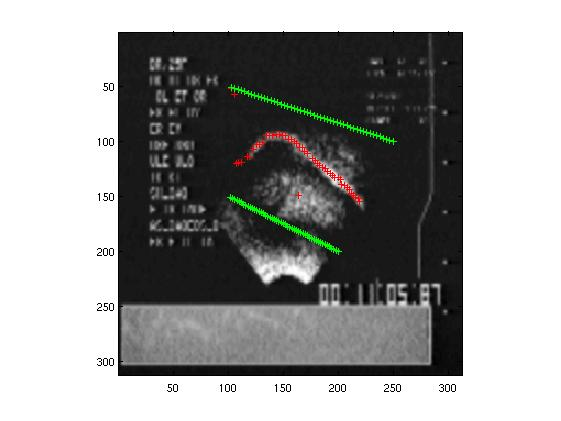
\includegraphics[width=500pt,height=400pt,scale=1]{small_values.jpg}
\newpage
\mbox{}
\newpage
\subsection{Contour initialisations}
\subsubsection{Higher Top Initial Contour}
The y of the top contour is decreased by 50.
$\lambda$=0.8 and M=100
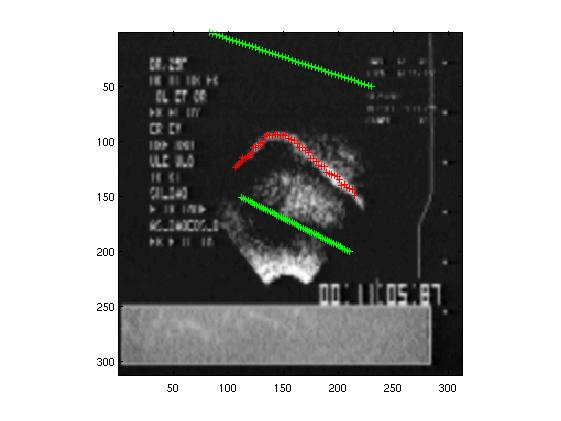
\includegraphics[width=500pt,height=400pt,scale=1]{top_plus_many.jpg}
\newpage
\mbox{}
\newpage
\mbox{}
\subsubsection{Lower Bottom Initial Contour}
The y of the top contour is decreased by 50.
$\lambda$=0.8 and M=100
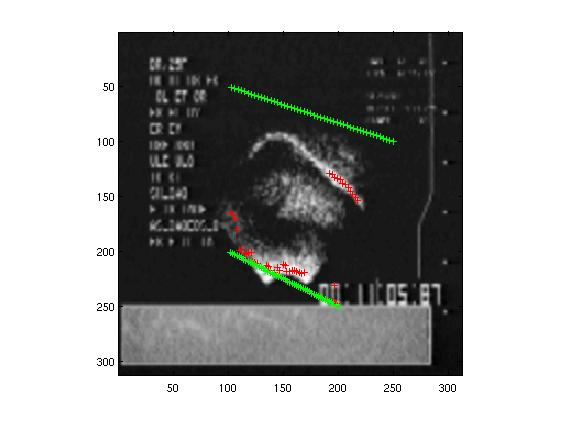
\includegraphics[width=500pt,height=400pt,scale=1]{bot_plus_50.jpg}	
\end{document}